\section{Related work}
\label{sec:relwork}

\paragraph{\textbf{Imperative probabilistic sequential programming languages and their semantics}}
Imperative probabilistic programs are the extension of conventional imperative programs with the capability to model randomness (typically from \emph{random number generators}), usually using a binary probabilistic choice construct~\cite{McIver2005bn,Hehner2011} or a random number generator (\emph{rand})~\cite{Hehner2004,Dahlqvist2020} sampling from the uniform distribution over a set (either finite or infinite). 
McIver and Morgan~\cite{McIver2020} show any discrete distribution, including uniform distributions, can be achieved through a binary probabilistic choice using a fair coin. Our work presented in this paper, ProbURel, uses both a probabilistic choice and a construct to draw a discrete uniform distribution from a finite set (similar to \emph{rand}).

The ``predicate style'' semantics (for example, weakest precondition~\cite{Dijkstra1976}, Hoare logic~\cite{Hoare1969}, and predicative programming~\cite{Hehner1984a}) for conventional imperative programs are boolean functions over state space. The semantics is sufficient to reason about these programs in the qualitative aspect, including termination or total correctness. Still, reasoning about probabilistic programs with natural quantitative measurements is insufficient. For this reason, boolean functions are generalised to real-valued functions over state space~\cite{Kozen1981,Kozen1985,McIver2005bn,Hehner2004}. 
One exception is the relational semantics~\cite{He2004} that embeds standard programs into the probabilistic world. In this semantics, probability distributions over states are captured in a special program variable ($prob$, a total function) in a standard program, and, therefore, the semantics of such probabilistic programs are still boolean functions over state space. Programs in our ProbURel are real-valued functions over state space.

Kozen's extension~\cite{Kozen1981,Kozen1985} replaced nondeterministic choice in conventional imperative programs with probabilistic choice, while McIver and Morgan~\cite{Morgan1999} added a probabilistic choice construct (and so it has both nondeterministic and probabilistic choice). McIver and Morgan's weakest pre-expectation or expectation transformer semantics~\cite{McIver2005bn}, the real-valued expressions over state space are called expectations (indeed random variables). The weakest pre-expectation expressed as $pre=wp\left(P, [post]\right)$ (where the square bracket $[\varg]$ converts a boolean-valued predicate to an arithmetic value, especially $[\ptrue]=1$ and $[\pfalse]=0$), is the least pre-expectations (evaluated in the initial state of $P$) to ensure that the probabilistic program $P$ terminates with post-expectation $[post]$ in its final state. % In other words, for $P$ to establish $post$ in its final state, the probability in its initial state is at least $pre$.
For example,  
\begin{align*}
    wp(x := x+1 _{(1/3)}\oplus x := x-1, [x \geq 0]) 
%= (1/3)*[x + 1 \geq 0] + (2/3)*[x - 1 \geq 0] 
%= (1/3)*[x \geq -1] + (2/3)*[x \geq 1] 
= (1/3)*[x = -1 \lor x = 0] + [x \geq 1] 
\end{align*}
means that in order for the program to establish $x \geq 0$, the probability of $x$ being $-1$ or $0$ (or $x \geq 1$, or $x < -1$) in its initial state is at least $1/3$ (or $1$, or $0$).
An extensive set of algebraic laws has been presented for reasoning about probabilistic programs, including loops and termination in~\cite[Appendix B]{McIver2005an}. 
Using this semantics, Kaminski~\cite{Kaminski2019a} developed an advanced weakest precondition calculus. {Based on the work, Schr\"oer et al.~\cite{Schroeer2023} developed a deductive verification infrastructure for verifying discrete probabilistic programs in terms of bounded expectations and expected runtimes, and termination probabilities using an intermediate verification language from which verification conditions are generated and verified in SMT solvers.} 
Our ProbURel uses a similar notation to the square bracket, called Iverson brackets. The predicates in ProbURel are UTP's alphabetised relations which have been used to establish program correctness using the weakest precondition calculus~\cite{Woodcock2004}. For this reason, our ProbURel can also describe the weakest pre-expectation semantics. 

The \emph{pGCL}~\cite{Morgan1999,McIver2005bn}, an extension of Dijkstra's Guarded Command Language (GCL)~\cite{Dijkstra1976} with a probabilistic choice construct, is a widely studied imperative probabilistic programming language. 
The weakest pre-expectation semantics is based on \emph{pGCL}. 
It is formalised in High-Order Logic (HOL)~\cite{Gordon1993} by Hurd et al.~\cite{Hurd2005} (based on the quantitative logic~\cite{Morgan1996a}), enabling verification of partial correctness of probabilistic programs, and also formalised in Isabelle/HOL by Cock~\cite{Cock2012} using shallow embedding (where probabilities are just primitive real numbers) to achieve improved proof automation.
The \emph{pGCL} has simple operational semantics~\cite{Gretz2014} using (parametric) Markov Decision Processes (MDPs) to establish a semantic connection with the weakest pre-expectation semantics and has relational semantics~\cite{Jifeng1997,He2004,Woodcock2019}, which is based on the theory of designs in UTP and mechanised in Isabelle/UTP~\cite{Ye2021}. The \emph{pGCL} contains a nondeterministic choice construct, but ProbURel in this paper does not include it. It is part of our future work to introduce nondeterminism. We also use Isabelle/UTP for automated verification, but the theory we use here is the theory of relations in UTP, which is more general than the theory of designs.

Probabilistic programs can be modelled as functions using a monadic interpretation. Hurd~\cite{Hurd2003} developed a formal HOL framework for modelling and verifying probabilistic algorithms using theorem proving. The work uses mathematical measure theory to represent probability space to model a random bit generator (an infinite stream of independent coin-flips). It uses a monadic state transformer to model probabilistic programs with higher-order logic functions. A probabilistic program consumes some bits from the front of the stream for randomisation and returns the remains. Audebaud et al.~\cite{Audebaud2009} use the monadic interpretation of randomised programs for probabilistic distributions (instead of measure theory) and mechanise their work in the Coq theorem prover~\cite{coq}. They consider probabilistic choice (without nondeterminism) in a functional language with recursion (instead of an imperative language). Programs in ProbURel are interpreted in imperative instead of monadic, and probabilistic loops are reasoned using fixed-point theories.

Dahlqvist et al.'s simple imperative probabilistic language~\cite{Dahlqvist2020} uses two constructs, $coin()$ and $rand()$, to introduce discrete and continuous uniform distributions, and both operational and denotational semantics are presented. In its operational semantics, a probabilistic program is assumed to start in two fixed infinite streams (one for $coin$ and one for $rand$), and the execution of each random sampling reads and removes the head from its corresponding stream. Eventually, the program is deterministic, and randomness is present in the infinite streams. This is similar to Hehner's probabilistic predicative programming~\cite{Hehner2004} where each call to $rand$ is stored in a mathematical variable (not a program variable). The denotational semantics of the simple language is given in terms of probability distributions. In ProbURel, we use a similar notation to $rand$ to draw a discrete uniform distribution from a finite set. The semantics of ProbURel are denotational.

Hehner~\cite{Hehner2004,Hehner2011} also generalises boolean functions for predicative programming to real-valued functions for probabilistic predicative programming. In his language, conditional and joint probability are modelled through sequential and parallel composition. One unique feature of the language is its capability to model epistemic uncertainty, due to the lack of knowledge of information and reducible after gaining more knowledge, and aleatoric uncertainty, due to the natural randomness of physical processes. Epistemic uncertainty is modelled through parallel composition using the subjective Bayesian approach. Our work, presented here, is based on Hehner's work. We formalise the syntax and semantics of the work, introduce UTP's alphabetised relations, bridge the semantics gap in dealing with probabilistic loops and mechanise it in Isabelle/UTP for automated reasoning.

Researchers also use Hoare logic to reason about probabilistic programs, such as the work presented in \cite{Ramshaw1979, 
    %\emph{pH}~\cite{
denHartog2002, 
Chadha2007}, and 
VPHL~\cite{Rand2015} uses a weighted tree structure to represent probability distributions in its semantics and can reason about the partial correctness of probabilistic programs. The probabilistic relational Hoare logic (pRHL)~\cite{Barthe2009} is a Hoare quadruple that establishes the equivalence of two programs and the usual Hoare logic to relate programs as pre- and post-conditions. {ELLORA~\cite{Barthe2018} is an assertion-based program logic for probabilistic programs and mechanised in the EasyCrypt theorem prover~\cite{Barthe2014}. The logic is presented in both abstract and concrete. The abstract logic is used for reasoning about loops and adversaries while the concrete logic facilitates formal verification. The logic features the reasoning of the broad class of loops for absolute termination, AST, and general termination using different assertions.} ProbURel uses UTP's alphabetised relations, which have been used to establish program correctness using Hoare logic~\cite{Woodcock2004}. For this reason, our ProbURel can also describe probabilistic Hoare logic semantics. The semantics of ProbURel are denotational, and two programs are equivalent if they are equal functions over the same state space.

\paragraph{\textbf{Recursion and Almost-sure termination}}
Reasoning about recursion is usually hard and is especially harder~\cite{Kaminski2019} for probabilistic programs because semantically probabilistic programs associate states with probability distributions other than merely boolean information for conventional programs. 
From this aspect, conventional programs can be regarded as a particular case of probabilistic programs where probability is always 1 or 0, so probabilistic programs are a more general paradigm. 

Morgan and McIver's early work~\cite{Morgan1996b,McIver2005an} uses general techniques invariants and variants for reasoning about loops. Invariants for probabilistic loops are now expectations. Variants {($V$)} are still integer-valued expressions but 
\begin{inparaenum}[a)]
\item {they are bounded below and above ($L \leq V < H$) by fixed integer constants ($L$ and $H$) if the states that satisfy the conjunction ($G \land Inv$) of the loop guard condition $G$ and the invariant $Inv$, are infinite}; 
\item for every iteration, there is a fixed non-zero probability $\varepsilon$ that the invariants are strictly decreased. 
\end{inparaenum}
A variant is not required always to be strictly decreased now; it could also be increased.
The variant rule is strengthened later by McIver et al. to remove the need to bound above, allow (quasi-) variants to be real-valued expressions, and $\varepsilon$ to vary~\cite[Theorem~4.1]{McIver2017}. Their new variant rule relies on a \emph{supermartingale}, a sequence of random variables (RVs) for which the expected value of the current random variable is larger than or equal to that of the subsequent random variable. Two parametric antitone functions characterise the quasi-variant called $p$ and $d$ for a lower bound $d$ on how much a program must decrease the variant with at least probability $p$. The new rule enables them to reason about the two-dimensional random walk, which is believed to be hard. % and cannot be proved by other approaches.
Chakarov et al.'s \emph{expectation invariants}~\cite{Chakarov2014} and Kaminski's \emph{sub-} and superinvariants~\cite{Kaminski2019a} are similar to Morgan and McIver's probabilistic invariants to use expectations for invariants. 
%uses a different terminology \emph{subinvariants} for Morgan and McIver's probabilistic invariants, and \emph{supvariants} for \emph{supermartingales}.
Our approach to reasoning about probabilistic loops is based on fixed-point theories, and the semantics of a loop is its unique fixed point when additional conditions are satisfied. We also use an iterative way to construct the fixed point, which is the supremum of an ascending chain.

As a consequence of the generality of probabilistic programs from conventional programs, it is much harder~\cite{Kaminski2015} to analyse the termination of probabilistic programs because now the program terminates with probability (instead of absolute termination~\cite{McIver2005an} for conventional programs). 
% See a talk "On Proving Almost-Sure Termination"  by Joost-Pieter Katoen on IFIP WG 2.2, 2019
The usual knowledge for conventional programs, such as termination or nontermination, finite run-time, and compositionality, is not valid for probabilistic programs. 
This problem has attracted a lot of interest in recent decades, such as~\cite{McIver2005an,Bournez2005,Esparza2012,Chakarov2013,FerrerFioriti2015,McIver2017,Agrawal2017,Huang2018,Chatterjee2018}. The research area of interest for probabilistic programs is a weakened termination, called \emph{almost-sure termination} (AST), or termination with probability one. In other words, a probabilistic program may not always terminate, but the probability of divergence is 0. For example, flipping a fair coin until the outcome is heads is such a program. 
As Esparza et al.~\cite{Esparza2012} pointed out, (conventional) termination is a purely topological property, namely the absence of cycles, while AST requires arithmetic reasoning. 
% usually not offered by termination provers.
Some recent studies have investigated the \emph{positive} almost-sure termination~\cite{Bournez2005} where probabilistic programs terminate in the finite expected time, and several studies have also assessed the \emph{null} almost-sure termination where probabilistic programs terminate almost-surely but not in the finite expected time. Hehner inspires our approach to reason about termination.

In Hehner's semantics~\cite{Hehner2011}, a time variable $t$ is introduced and is strictly increased in each iteration of a loop. For example, it can be an extended integer number (including $\infty$ for nontermination) and is used to count iterations. His approach~\cite{Hehner1999} for termination of (probabilistic) loops is stronger than total correctness (equal to partial correctness plus termination) because the time variable allows reasoning about not only whether a loop terminates but also when it terminates (run-time analysis). One example from his paper is a probabilistic loop about throwing a pair of dice till they have the same outcome.
The invariant (or hypothesis) of this loop, shown below and proved in Sect.~\ref{sec:ex_cases:dice}, gives the distribution of final states (primed variables).
\begin{align*}
    & H \defs {\ibracket{d_1' = d_2'} * \ibracket{t' \geq t + 1} * {\left(\frac{5}{6}\right)^{\left(t' - t - 1\right)}} * \left(\frac{1}{36}\right)}
\end{align*} 
We are interested in the probability distribution in terms of iterations or $t$, and so we substitute $\ibracket{d_1' = d_2'}$ with 6 because there are 6 possible combinations of $d_1'$ and $d_2'$ in each experiment to have them equal. 
\begin{align*}
    & Ht \defs {6 * \ibracket{t' \geq t + 1} * {\left(\frac{5}{6}\right)^{\left(t' - t - 1\right)}} * \left(\frac{1}{36}\right)} = {\ibracket{t' \geq t + 1} * {\left(\frac{5}{6}\right)^{\left(t' - t - 1\right)}} * \left(\frac{1}{6}\right)}
\end{align*} 
Provided the initial value of $t$ is 0, we plot the program's termination probability using this invariant in Fig.~\ref{fig:dice_t_prob}. Because $t$ counts iterations, the diagram also shows the probability of the termination in the exact iteration $t$. The probability for $t'=1$ is $1/6$ ($\approx 0.167$), so the program terminates in the first iteration with probability $1/6$ as expected ($6$ among total $6*6=36$ combinations).
%\begin{tikzpicture}[ybar]
%  \draw[color=red,fill=red!80,bar width=6pt]
%    plot coordinates{(0,1) (.5,1.2) (1,.6) (1.5,.7) (2,.9)};
%  \draw[color=red!50,fill=red!20,bar width=4pt,bar shift=3pt]
%    plot coordinates{(0,1.2) (.5,1.3) (1,.5) (1.5,.2) (2,.5)};
%\end{tikzpicture}

\begin{figure}[!ht]
    \begin{center}
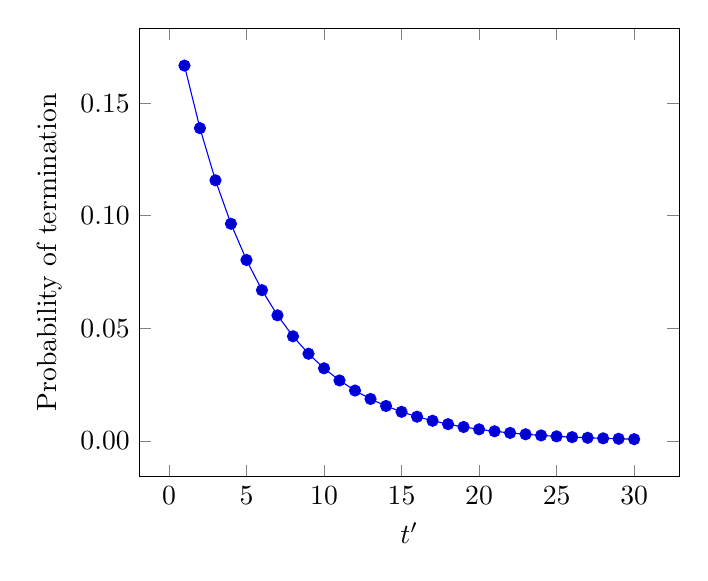
\begin{tikzpicture}
\begin{axis}[%[ybar] 
    xlabel={$t'$},
    ylabel={Probability of termination},
    y tick label style={/pgf/number format/.cd,fixed,fixed zerofill,precision=2},
]
    \addplot table[header=false,col sep=&,row sep=\\,y expr={\thisrowno{1}}] {
        1 & 1/6\\
        2 & (1/6)*(5/6)\\
        3 & (1/6)*(5/6)^2\\
        4 & (1/6)*(5/6)^3\\
        5 & (1/6)*(5/6)^4\\
        6 & (1/6)*(5/6)^5\\
        7 & (1/6)*(5/6)^6\\
        8 & (1/6)*(5/6)^7\\
        9 & (1/6)*(5/6)^8\\
        10& (1/6)*(5/6)^9\\
        11& (1/6)*(5/6)^10\\
        12& (1/6)*(5/6)^11\\
        13& (1/6)*(5/6)^12\\
        14& (1/6)*(5/6)^13\\
        15& (1/6)*(5/6)^14\\
        16& (1/6)*(5/6)^15\\
        17& (1/6)*(5/6)^16\\
        18& (1/6)*(5/6)^17\\
        19& (1/6)*(5/6)^18\\
        20& (1/6)*(5/6)^19\\
        21& (1/6)*(5/6)^20\\
        22& (1/6)*(5/6)^21\\
        23& (1/6)*(5/6)^22\\
        24& (1/6)*(5/6)^23\\
        25& (1/6)*(5/6)^24\\
        26& (1/6)*(5/6)^25\\
        27& (1/6)*(5/6)^26\\
        28& (1/6)*(5/6)^27\\
        29& (1/6)*(5/6)^28\\
        30& (1/6)*(5/6)^29\\
    };
  \end{axis}
\end{tikzpicture}
    \end{center}
    \caption{Termination probability over $t'$ for dice.}
    \label{fig:dice_t_prob}
\end{figure}

Reasoning about almost-sure termination becomes an arithmetic summation of this distribution, as shown below, which sums to 1.
\begin{align*}
\displaystyle\sum_{t'=0}^{\infty} \ibracket{t' \geq 1} * {\left(\frac{5}{6}\right)^{\left(t' - 1\right)}} * \left(\frac{1}{6}\right) 
    = \sum_{t'=1}^{\infty} {\left(\frac{5}{6}\right)^{\left(t' - 1\right)}} * \left(\frac{1}{6}\right) 
    =  \left(\frac{1}{6}\right) * \sum_{t'=1}^{\infty} {\left(\frac{5}{6}\right)^{\left(t' - 1\right)}}
    = 1.0
\end{align*}
\noindent
The expected run-time is the expectation of $t'$, simply the sequential composition of $\left(Ht ; t'\right) = t + 6$, denoting, on average, it takes six throws to have their outcomes equal.

% \cite{Kaminski2019a} use Kleene fixed-point theorem.
%\paragraph{Automated verification}
% Model checking is a widely applied verification technique to analyse probabilistic systems, supported in probabilistic model checkers such as PRISM~\cite{Kwiatkowska2011}, Storm~\cite{Dehnert2017}, and MODEST Toolset.\footnote{\url{www.modestchecker.net/}}.
% Formal verification of probabilistic programs or algorithms using theorem proving~\cite{Hurd2003,Hurd2005}.
% 
% McIver et al. presented probabilistic Kleene algebra~\cite{McIver2005a}, \emph{pKA}, for automated reasoning support and mechanisation of automated counterexample search in Isabelle/HOL. The \emph{pKA} was also extended with the generalisation of separation theorems~\cite{Cohen2000} to reduce the complexity of algebraic reasoning by separating interleaving behaviours of probabilistic systems~\cite{McIver2006}. 
% 
{
\paragraph{\textbf{Summary}}
\begin{table*}[ht]
    \caption{{Comparison of different probabilistic semantics}}
    \label{tab:related_work}\centering
\bgroup
\def\arraystretch{1.0}
\setlength\tabcolsep{.5mm}
    \begin{tabular}{@{}l c cccccc c ccccc c cccc c c c @{}}
        \toprule
        \multirow{2}{*}{Approach} & %\phantom{a} 
        & \multicolumn{6}{c}{Modelling features} & \phantom{a} & \multicolumn{3}{c}{Advanced} & \phantom{a} & \multicolumn{5}{c}{Reasoning and Verification} & %\phantom{a} 
        & \multirow{2}{*}{Auto} \\
        \cmidrule{3-8} \cmidrule{10-12} \cmidrule{14-18}
        &
        & PrCh & UniD 
        & Cond
        & Jnt & NonD 
        & Expr
        & 
        % Advanced
        & Para & Unf & Refn & 
        %Verification
        & WP & ExaPD & ExpRT 
        & Inv & 
        Para &
        \\
        \midrule
        %Synchronous Timed AD
        PPDL\cite{Kozen1985} & 
             & \checkmark & \checkmark & &  &  & Bsc & & &  &  & 
             & & \checkmark & \checkmark & \checkmark & & & \\
        WPE\cite{McIver2005} & 
             & \checkmark & & &  & \checkmark & Bsc & 
             & &  & \checkmark &  
             & \checkmark & & & \checkmark & & & \autotp \\
        AWPE\cite{Kaminski2019a} & 
             & \checkmark & \checkmark & \checkmark &  & \checkmark & Bsc & 
             & &  & \checkmark &  
             & \checkmark & & \checkmark & \checkmark & & & \checkmark \\
        DVWPE\cite{Schroeer2023} & 
             & \checkmark & \checkmark & \checkmark &  & \checkmark & Bsc & 
             & &  & &  
             & \checkmark & & \checkmark & \checkmark & & & \checkmark \\
        ELLORA\cite{Barthe2018} & 
             & \checkmark & \checkmark & & & & Bsc & 
             & & & & 
             & ASS & \checkmark & \checkmark & \checkmark & & & \autotp \\
        PDs\cite{He2004} & 
             & \checkmark & & &  & \checkmark & Rich & 
             & \checkmark & \checkmark & \supportnoimpl  & 
             & CTr & \checkmark &  & \checkmark  & \checkmark & & \autotp \\
        PPP\cite{Hehner2004} & 
            & \checkmark & \checkmark & \checkmark & \checkmark&  & Bsc & 
            & & & \supportnoimpl & 
            & & \checkmark & \checkmark & \checkmark & & &  \\ 
        Our & 
            & \checkmark & \checkmark & \checkmark & \checkmark&  & Rich & 
            & \checkmark & \checkmark & \supportnoimpl & 
            & \supportnoimpl & \checkmark & \checkmark & \checkmark & \checkmark & & \autotp \\ 
        \midrule
        \multicolumn{20}{p{1.0\linewidth}}{\textbf{Acronym}: 
            ASS: assertion-based;
            Auto: automation;
            AWPE: advanced WPE;
            Bsc: basic;
            CTr: contract-based;
            Cond: conditional probability;
            DVWPE: WPE-based deductive verification infrastructure;
            ExaPD: exact probability distributions;
            Exp: expression and type system; 
            ExpRT: expected runtime;
            Inv: loop invariant; 
            Jnt: joint probability, especially supporting general likelihood functions; 
            NonD: nondeterministic choice;
            Para: parametric models or reasoning;
            PDs: probabilistic designs; 
            PrCh: probabilistic choice; 
            Refn: refinement; 
            TP: theorem proving;
            Unf: unification; 
            UniD: construct for uniform distributions;
            \supportnoimpl: supported but not yet developed;
            %\supportneedext: supported but need further development;
            %\partially: partially (supported in some stages but not in all stages), or claimed to support but no further details disclosed;
            \autotp: automation through theorem proving; 
        } \\
        \bottomrule
\end{tabular}
\egroup
\end{table*}

In Table~\ref{tab:related_work}, we summarise the comparison of different probabilistic semantics in terms of four perspectives: modelling features, advanced features, reasoning and verification, and automation. In modelling features, we consider the support of constructs for usual probabilistic choice, uniform distributions, conditioning, joint probability, nondeterministic choice, and expression and type systems. Our work supports all but nondeterminism. Notably, our language has a rich expression and type system which is based on the Z notation~\cite{Spivey1992,Woodcock1996} and the mechanised Z mathematical toolkit\footnote{\url{https://github.com/isabelle-utp/Z_Toolkit}.} in Isabelle/HOL, which entitles us to model abstract probabilistic programs and capture rich semantics. Our language and semantic framework can support parametric models, is able to unify other semantics and support refinement thanks to our UTP relations. Probabilistic designs are also based on UTP and so the theory supports similar features as ours. In terms of verification, our work can be used to unify the WPE semantics (but this needs the new development), and support parametric verification. 
}
